\section{Ocean Dissipation in Enceladus \label{sec:results_Enceladus}}

\subsection{Rayleigh Friction} \label{sec:ray_enc}

As with our Titan results, we calculated globally averaged surface heat flux for over 3000 simulations in the $h$-$\alpha$ parameter space. These results are shown for the eccentricity and obliquity tides in Figure \ref{fig:linEncel}.

There are several more gravity wave resonances found for Enceladus than Titan in both tidal components, as shown in Figure \ref{fig:lincEccEncel}. The eccentricity tide excites resonances at \SIlist{1.3;1.9;3.8;8.7;29;50;360}{m}; a total of 7 resonances, whereas Titan only has 3 (Figure \ref{fig:lincEccTitan}). By solving the LTEs using both the eccentricity-radial and libration tides simultaneously, we capture any coupling these two tidal components may initiate in the ocean flow and find no new resonances. Increasing the resolution of the parameter space would almost certainly reveal more resonances, but this is only likely for oceans with $h_0 <$ \SI{10}{\metre}. 

The most dissipative eccentricity tide resonance is also the deepest, with an average surface heat flux of \SI{4.6}{\watt\per\square\metre} at $\alpha\sim$ \SI{2e-6}{\per\second}, three orders of magnitude greater than Titan's largest resonance. This is equivalent to a total power output of $\sim$ \SI{3610}{\giga\watt}, well in excess of the observed value of (at least) \SI{5}{\giga\watt} by two to three orders of magnitude \citep{spencer2006cassini,howett2011high, spencer2013new}.  

\begin{figure}[!t]
    \centering
    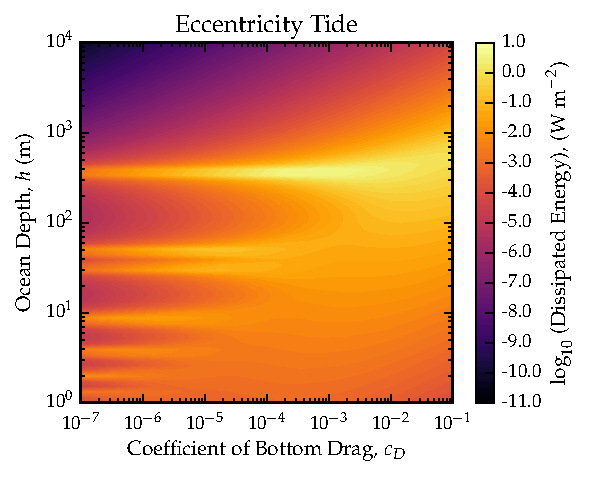
\includegraphics[width=\linewidth]{Figures/enceladus_bottom}
\caption{As for Figure \ref{fig:linEncel}, but for the bottom drag regime. The obliquity tide is also ignored. \label{fig:botEncel}}
\end{figure}

The stark colour difference between the eccentricity and obliquity tide plots in Figure \ref{fig:linEncel} is a result of Enceladus' negligible obliquity ($\theta_0 \sim$ \num{e-4} degrees \citep{chen2013tidal, baland2016obliquity}). This causes average surface dissipation to range from \SIrange{e-7}{e-14}{\watt\per\square\metre} over our explored parameter space, which has an almost negligible effect on the thermal and orbital evolution of the satellite. Gravity wave resonances are found at \SIlist{1.6;2.7;5.5;18;160}{\metre}, with the characteristic Rossby wave resonance extending diagonally across the parameter space from around $h=$ \SI{500}{\metre}.

Away from shallow oceans, we once again find excellent agreement between the numerical and semi-analytical solutions from \citet{matsuyama2014tidal} in terms of both the resonant ocean thicknesses and magnitude of the dissipation. Much of the parameter space has a discrepancy of $<$ \SIrange{1}{5}{\percent}, with this increasing to $\sim$ \SI{10}{\percent} for resonances. As demonstrated in Figure \ref{fig:conv}, this can easily be decreased with higher resolution simulations, at the expense of computational run time.


\subsection{Bottom Friction}

We neglect running the obliquity tide bottom drag case for Enceladus. As mentioned in the previous section, the obliquity of Enceladus is close to Cassini State \citep{chen2011obliquity,chen2013tidal}, making tidal flow and dissipation from obliquity negligible. Additionally, the low drag experienced due to weak obliquity tide flow leads to long simulation run times in order to achieve equilibrium, which is a severe challenge numerically.

Bottom drag results for the eccentricity tide on Enceladus are shown in Figure \ref{fig:botEncel}. The gravity wave resonances are found at identical ocean thicknesses to the Rayleigh drag results in Figure \ref{fig:lincEccEncel}. There is, however, a much greater contrast in dissipation magnitude in this parameter space when compared to the Rayleigh drag results. Dissipation drops off rapidly by many orders of magnitude with increasing ocean depth away from the \SI{360}{\metre} resonance. This is expected given the velocity squared dependence in the bottom drag term in Equation \ref{eq:mom}. 

\subsection{Comparison with Scaling Laws}

\begin{figure}[!b]
\centering
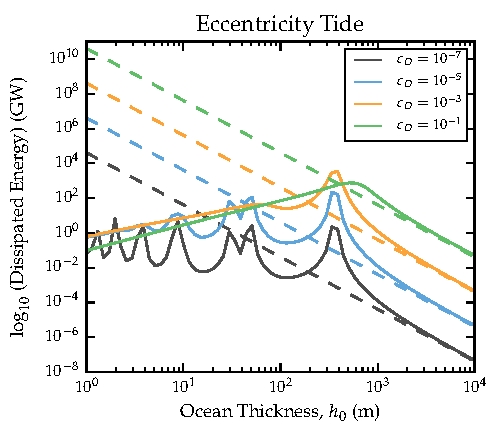
\includegraphics[width=0.85\linewidth]{Figures/enceladus_scaling}
\caption{Comparison of the ODIS numerical results (solid lines) and those calculated using the scaling laws (dashed lines) derived in \citet{chen2013tidal}, for Enceladus under the eccentricity tide. The colours represent different values of bottom drag coefficient. \label{fig:scalEncel}}
\end{figure}

The bottom drag eccentricity tide results for Enceladus are compared to \citet{chen2013tidal} scaling laws in Figure \ref{fig:scalEncel}. As was the case with Titan, we find poor agreement for resonant ocean configurations, with increasingly good agreement away from resonances. The scaling laws cannot take into account the resonant ocean configurations due to the non-linearity of these features. However, the general trend of decreasing dissipation with increasing ocean depth is captured by the scaling laws and agrees well with our numerical results. This agreement provides further validation to the numerical model and techniques employed in this work.

\subsection{Implications for Enceladus}

Eccentricity is the only significant contributor to ocean dissipation in Enceladus. Under both Rayleigh and bottom drag, the deepest occurring gravity wave resonance can easily account for the observed SPT power output \citep{spencer2006cassini,howett2011high,spencer2013new}. However, this resonance is relatively shallow. Of course, Enceladus' ocean depth is unconstrained, although non-unique gravity modelling is consistent with an ocean on the order of \SI{10}{\kilo\metre} thick, at least under the SPT \citep{iess2014gravity}. Thus, based on our results, we expect that ocean dissipation is insignificant over long time scales for Enceladus. 
%Resonant ocean configurations occur only for shallow oceans under the eccentricity tide and obliquity tide flow is negligible, meaning dissipation is minimal over the vast majority of the likely parameter space.

The numerical model has also revealed no new resonances in either Rayleigh or bottom drag by applying both the eccentricity-radial and eccentricity-libration tide simultaneously, a technique that is not possible analytically.

The amplitude of forced libration on Enceladus \citep{thomas2015enceladus}, as well as the negative mass anomaly observed at the SPT \citep{iess2014gravity, mckinnon2015effect} indicate that its subsurface ocean is global in extent and deeper beneath the SPT. This variable ocean thickness is neglected in our model, and may lead to localised heating at the boundary between shallow and deep oceans. The effect on resonance ocean configurations is unknown. Incorporating a variable ocean thickness into the LTEs is only possible numerically, and will be one focus of future work.


